\documentclass{beamer}

\usetheme{Boadilla}

\usepackage[utf8]{inputenc}
\usepackage[english]{babel}
\usepackage{multicol} % itemize sur plusieurs colonnes
\usepackage{tikz} % pour tracer des figures
\usepackage{subfig} % pour mettre images à côté
\usepackage[absolute,overlay]{textpos}
\setcounter{tocdepth}{1} % afficher que les sections dans le sommaire
\usepackage{changepage}
\usepackage{xcolor} % to highlight text
\usepackage{ulem} % strikeout text
\usepackage[export]{adjustbox} % center images and text in table
\usepackage{array}
\newcolumntype{?}{!{\vrule width 1pt}}

\setbeamertemplate{navigation symbols}{}

\hypersetup{ % couleur des liens
    colorlinks=true,
    linkcolor=blue,
    filecolor=black,      
    urlcolor=blue,
}

\AtBeginSection[] % faire apparaître le sommaire avant chaque nouvelle section
{
  \begin{frame}
    \frametitle{Plan}
    \tableofcontents[currentsection]
  \end{frame}
}

\newenvironment{myitemize}
{ \begin{itemize}
	\scriptsize }
{ \end{itemize} } 

\newif\ifplacelogo %Booléen pour placer ou non le logo
\placelogotrue %Initialisation booléen à 'True'
\logo{\ifplacelogo
\includegraphics[height=5mm]{Images/logoINSA.png}\fi} %Initialisation du logo (fonction du booléen)

\title{Animal Classification with Keras}
\author[MA \--- DT \--- WZ]{Mehdi ABOUZAID  \\ Damien TOOMEY \\ Weihao ZHOU}
\institute[INSA Rouen]{INSA \--- National Institute of Applied Sciences}
\date{\today}

\begin{document}

\begin{frame}
\titlepage
\end{frame}

\placelogofalse
\begin{frame}
\frametitle{Plan} 
\tableofcontents
\end{frame}	

\section{Introduction}
\definecolor{red}{rgb}{1,0,0}
\definecolor{green}{rgb}{0,0.39,0}
\renewcommand{\arraystretch}{1.1}
\setlength{\tabcolsep}{2pt} % spacing between columns

\subsection{Some information}
\begin{frame}
\frametitle{Introduction}
\framesubtitle{Some information}

\begin{textblock}{15}(7.67,-0.62)
	\begin{figure}[H]
		
\includegraphics[width=0.1\textwidth]{Images/Team/MehdiABOUZAID.png} 
	\end{figure}
\end{textblock}

\begin{itemize}
\item[•] Article:
\item[] \textsl{Animal Recognition and Identification with Deep Convolutional Neural
Networks for Automated Wildlife Monitoring}
\item[•] Studied models:
\end{itemize}

\begin{adjustwidth}{-1.5em}{-1.5em}
\begin{center}
{\fontsize{9.5}{15}\selectfont
\begin{tabular}{|c|c|c|c|c|c|}
\cline{5-6}
\multicolumn{4}{c|}{} & \multicolumn{2}{c|}{\textit{Validation Set}} \\
\cline{2-6}
\multicolumn{1}{c|}{} & \textbf{ILSVRC} & \textbf{Parameters} & \textbf{Trainable Layers} & \textbf{Top-1 Accuracy} & \textbf{Top-5 Accuracy} \\
\hline
AlexNet & 2012 & 62,378,344 & 8 & 0.633 & 0.846 \\
\hline
VGG-16 & 2014 & 138,357,544 & 16 & 0.713 & 0.901 \\
\hline
ResNet-50 & 2015 & 25,636,712 & 50 & 0.749 & 0.921 \\
\hline
Xception & 2017 & 22,910,480 & 71 & 0.790 & 0.945 \\
\hline
\end{tabular}
}
\end{center}
\end{adjustwidth}

\begin{itemize}
\item[•] Vocabulary:
\item[] kernel = filter = receptive field = mask
\end{itemize}

\end{frame}

\subsection{Some information}
\begin{frame}
\frametitle{Introduction}
\framesubtitle{Our dataset} 

\begin{textblock}{15}(7.67,-0.62)
	\begin{figure}[H]
		
\includegraphics[width=0.1\textwidth]{Images/Team/MehdiABOUZAID.png} 
	\end{figure}
\end{textblock}

\setlength{\tabcolsep}{10pt} % spacing between columns
\begin{center}
\begin{tabular}{ccc}
\textbf{Input} & \textbf{Output} & \textbf{Number of Images} \\
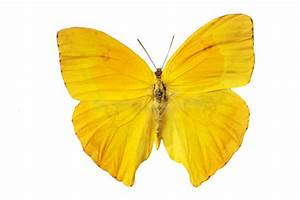
\includegraphics[valign=m,width=0.29\textwidth]{Images/Dataset/butterfly.jpeg} & butterfly & 1991 \\
\vspace{0.1cm}
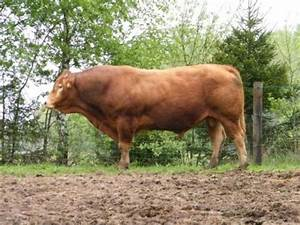
\includegraphics[valign=m,width=0.29\textwidth]{Images/Dataset/cow.jpeg} & cow & 2039 \\
\vspace{0.1cm}
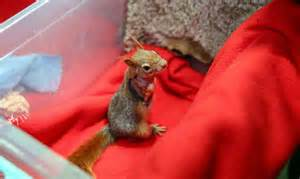
\includegraphics[valign=m,width=0.29\textwidth]{Images/Dataset/squirrel.jpeg} & squirrel & 2013  \\
\end{tabular}
\end{center}		 

\end{frame}

\section{CNN}
\begin{frame}
\frametitle{CNN: VGG-16 as example}
\framesubtitle{Input} 

\begin{textblock}{15}(7.67,-0.62)
	\begin{figure}[H]
		
\includegraphics[width=0.1\textwidth]{Images/Team/DamienTOOMEY.png} 
	\end{figure}
\end{textblock}

\begin{adjustwidth}{-1.5em}{-1.5em}
\setlength\arraycolsep{2pt}

\[ \overbrace{\begin{array}{ccc}
\begin{pmatrix}
R_{1,1} & R_{1,2} & R_{1,3} & R_{1,4} \\
R_{2,1} & R_{2,2} & R_{2,3} & R_{2,4} \\
R_{3,1} & R_{3,2} & R_{3,3} & R_{3,4} \\
R_{4,1} & R_{4,2} & R_{4,3} & R_{4,4} \\
\end{pmatrix}
& \begin{pmatrix}
G_{1,1} & G_{1,2} & G_{1,3} & G_{1,4} \\
G_{2,1} & G_{2,2} & G_{2,3} & G_{2,4} \\
G_{3,1} & G_{3,2} & G_{3,3} & G_{3,4} \\
G_{4,1} & G_{4,2} & G_{4,3} & G_{4,4} \\
\end{pmatrix}
& \begin{pmatrix}
B_{1,1} & B_{1,2} & B_{1,3} & B_{1,4} \\
B_{2,1} & B_{2,2} & B_{2,3} & B_{2,4} \\
B_{3,1} & B_{3,2} & B_{3,3} & B_{3,4} \\
B_{4,1} & B_{4,2} & B_{4,3} & B_{4,4} \\
\end{pmatrix} \\
& \textcolor{white}{phantom} & \\
\mathcal{I}_{\textcolor{red}{red}} & \mathcal{I}_{\textcolor{green}{green}} & \mathcal{I}_{\textcolor{blue}{blue}} \\
\end{array}}^{\mathcal{I} = \begin{pmatrix}
I_{1,1} & I_{1,2} & I_{1,3} & I_{1,4} \\
I_{2,1} & I_{2,2} & I_{2,3} & I_{2,4} \\
I_{3,1} & I_{3,2} & I_{3,3} & I_{3,4} \\
I_{4,1} & I_{4,2} & I_{4,3} & I_{4,4} \\
\end{pmatrix}}
\]

\end{adjustwidth}
\end{frame}


\begin{frame}
\frametitle{CNN: VGG-16 as example}
\framesubtitle{2D Convolution : only \textbf{3x3 kernel}, \textbf{stride 1}, \textbf{zero padding of thickness 1}} 

\begin{textblock}{15}(7.67,-0.62)
	\begin{figure}[H]
		
\includegraphics[width=0.1\textwidth]{Images/Team/DamienTOOMEY.png} 
	\end{figure}
\end{textblock}

\begin{adjustwidth}{-1.5em}{-1.5em}
\setlength\arraycolsep{2pt}
{\fontsize{9.5}{10}\selectfont
\[
\begin{array}{ccc}
\mathcal{I}_{\textcolor{red}{red}} & \mathcal{I}_{\textcolor{green}{green}} & \mathcal{I}_{\textcolor{blue}{blue}} \\
& \textcolor{white}{phantom} & \\
\begin{pmatrix}
{\only<1,3>{0}}{\only<2>{\color{red}\textbf{0}}} & {\only<1>{0}}{\only<2,3>{\color{red}\textbf{0}}} & {\only<1>{0}}{\only<2,3>{\color{red}\textbf{0}}} & {\only<1,2>{0}}{\only<3>{\color{red}\textbf{0}}} & 0 & 0 \\
{\only<1,3>{0}}{\only<2>{\color{red}\textbf{0}}} & {\only<1>{R_{1,1}}}{\only<2,3>{\color{red}\textbf{$R_{1,1}$}}} & {\only<1>{R_{1,2}}}{\only<2,3>{\color{red}\textbf{$R_{1,2}$}}} & {\only<1,2>{R_{1,3}}}{\only<3>{\color{red}\textbf{$R_{1,3}$}}} & R_{1,4} & 0 \\
{\only<1,3>{0}}{\only<2>{\color{red}\textbf{0}}} & {\only<1>{R_{2,1}}}{\only<2,3>{\color{red}\textbf{$R_{2,1}$}}} & {\only<1>{R_{2,2}}}{\only<2,3>{\color{red}\textbf{$R_{2,2}$}}} & {\only<1,2>{R_{2,3}}}{\only<3>{\color{red}\textbf{$R_{2,3}$}}} & R_{2,4} & 0 \\
0 & R_{3,1} & R_{3,2} & R_{3,3} & R_{3,4} & 0 \\
0 & R_{4,1} & R_{4,2} & R_{4,3} & R_{4,4} & 0 \\
0 & 0 & 0 & 0 & 0 & 0\\
\end{pmatrix}
& \begin{pmatrix}
{\only<1,3>{0}}{\only<2>{\color{green}\textbf{0}}} & {\only<1>{0}}{\only<2,3>{\color{green}\textbf{0}}} & {\only<1>{0}}{\only<2,3>{\color{green}\textbf{0}}} & {\only<1,2>{0}}{\only<3>{\color{green}\textbf{0}}} & 0 & 0 \\
{\only<1,3>{0}}{\only<2>{\color{green}\textbf{0}}} & {\only<1>{G_{1,1}}}{\only<2,3>{\color{green}\textbf{$G_{1,1}$}}} & {\only<1>{G_{1,2}}}{\only<2,3>{\color{green}\textbf{$G_{1,2}$}}} & {\only<1,2>{G_{1,3}}}{\only<3>{\color{green}\textbf{$G_{1,3}$}}} & G_{1,4} & 0 \\
{\only<1,3>{0}}{\only<2>{\color{green}\textbf{0}}} & {\only<1>{G_{2,1}}}{\only<2,3>{\color{green}\textbf{$G_{2,1}$}}} & {\only<1>{G_{2,2}}}{\only<2,3>{\color{green}\textbf{$G_{2,2}$}}} & {\only<1,2>{G_{2,3}}}{\only<3>{\color{green}\textbf{$G_{2,3}$}}} & G_{2,4} & 0 \\
0 & G_{3,1} & G_{3,2} & G_{3,3} & G_{3,4} & 0 \\
0 & G_{4,1} & G_{4,2} & G_{4,3} & G_{4,4} & 0 \\
0 & 0 & 0 & 0 & 0 & 0 \\
\end{pmatrix}
& \begin{pmatrix}
{\only<1,3>{0}}{\only<2>{\color{blue}\textbf{0}}} & {\only<1>{0}}{\only<2,3>{\color{blue}\textbf{0}}} & {\only<1>{0}}{\only<2,3>{\color{blue}\textbf{0}}} & {\only<1,2>{0}}{\only<3>{\color{blue}\textbf{0}}} & 0 & 0 \\
{\only<1,3>{0}}{\only<2>{\color{blue}\textbf{0}}} & {\only<1>{B_{1,1}}}{\only<2,3>{\color{blue}\textbf{$B_{1,1}$}}} & {\only<1>{B_{1,2}}}{\only<2,3>{\color{blue}\textbf{$B_{1,2}$}}} & {\only<1,2>{B_{1,3}}}{\only<3>{\color{blue}\textbf{$B_{1,3}$}}} & B_{1,4} & 0 \\
{\only<1,3>{0}}{\only<2>{\color{blue}\textbf{0}}} & {\only<1>{B_{2,1}}}{\only<2,3>{\color{blue}\textbf{$B_{2,1}$}}} & {\only<1>{B_{2,2}}}{\only<2,3>{\color{blue}\textbf{$B_{2,2}$}}} & {\only<1,2>{B_{2,3}}}{\only<3>{\color{blue}\textbf{$B_{2,3}$}}} & B_{2,4} & 0 \\
0 & B_{3,1} & B_{3,2} & B_{3,3} & B_{3,4} & 0 \\
0 & B_{4,1} & B_{4,2} & B_{4,3} & B_{4,4} & 0 \\
0 & 0 & 0 & 0 & 0 & 0 \\
\end{pmatrix} \\
& \textcolor{white}{phantom} & \\
Kernel[:,:,0] & Kernel[:,:,1] & Kernel[:,:,2] \\
\begin{bmatrix}
w_1 & w_2 & w_3 \\
w_4 & w_5 & w_6 \\
w_7 & w_8 & w_9
\end{bmatrix}
& \begin{bmatrix}
w_{10} & w_{11} & w_{12} \\
w_{13} & w_{14} & w_{15} \\
w_{16} & w_{17} & w_{18}
\end{bmatrix}
& \begin{bmatrix}
w_{19} & w_{20} & w_{21} \\
w_{22} & w_{23} & w_{24} \\
w_{25} & w_{26} & w_{27}
\end{bmatrix}
\end{array} 
\]
}


{\only<1>{
\vspace{0.2cm}
\begin{center}
Goal : learn the weights in the kernels
\end{center}	
}}

{\only<2,3>{
{\fontsize{10}{0}\selectfont
\begin{align*}
& w = np.hstack((Kernel[:,:,0].flatten(), Kernel[:,:,1].flatten(), Kernel[:,:,2].flatten())) \\
& \\
& x = np.hstack((\textcolor{red}{Window}.flatten(),\textcolor{green}{Window}.flatten(),\textcolor{blue}{Window}.flatten())) \\
& \\
& {\only<2>{FeatureMap[0,0,0] = ReLU(w.dot(x) + bias) = ReLU(w^T x + bias)}}{\only<3>{FeatureMap[1,0,0] = ReLU(w.dot(x) + bias) = ReLU(w^T x + bias)}}
\end{align*}
}
}}
\end{adjustwidth}
\end{frame}

\begin{frame}
\frametitle{CNN: VGG-16 as example}
\framesubtitle{Feature maps \& Max pooling} 

\begin{textblock}{15}(7.67,-0.62)
	\begin{figure}[H]
		
\includegraphics[width=0.1\textwidth]{Images/Team/DamienTOOMEY.png} 
	\end{figure}
\end{textblock}

\begin{itemize}
\item[•] as many feature maps as there are kernels
\item[•] each kernel is detecting a particular feature (edges,texture,...)
\item[•] by adding more kernels, the model can learn to detect more complex features
\item[•] max pooling $ \Rightarrow $ shrinking of the feature maps 
\begin{itemize}
\item[-] no learnable parameters
\item[-] 2x2 kernel
\item[-] stride 2
\item[-] no zero padding
\end{itemize}
\end{itemize}

\[
\begin{pmatrix}
\textcolor{red}{1} & \textcolor{red}{1} & \textcolor{green}{2} & \textcolor{green}{4} \\
\textcolor{red}{5} & \textcolor{red}{6} & \textcolor{green}{7} & \textcolor{green}{8} \\
3 & 2 & \textcolor{blue}{1} & \textcolor{blue}{0} \\
1 & 2 & \textcolor{blue}{3} & \textcolor{blue}{4} \\
\end{pmatrix}
\underbrace{\rightarrow}_{\text{max pooling}}
\begin{pmatrix}
\textcolor{red}{6} & \textcolor{green}{8} \\
3 & \textcolor{blue}{4} \\
\end{pmatrix}
\]

\end{frame}

\begin{frame}
\frametitle{CNN: VGG-16 as example}
\framesubtitle{Bias} 

\begin{textblock}{15}(7.67,-0.62)
	\begin{figure}[H]
		
\includegraphics[width=0.1\textwidth]{Images/Team/DamienTOOMEY.png} 
	\end{figure}
\end{textblock}

\[ weighted\_sum = \sum_{i=1}^n w_i x_i = w^T x \]

\begin{itemize}
\item[•] biases are learned parameters
\item[•] each neuron has a bias
\end{itemize}

\begin{figure}[H]
	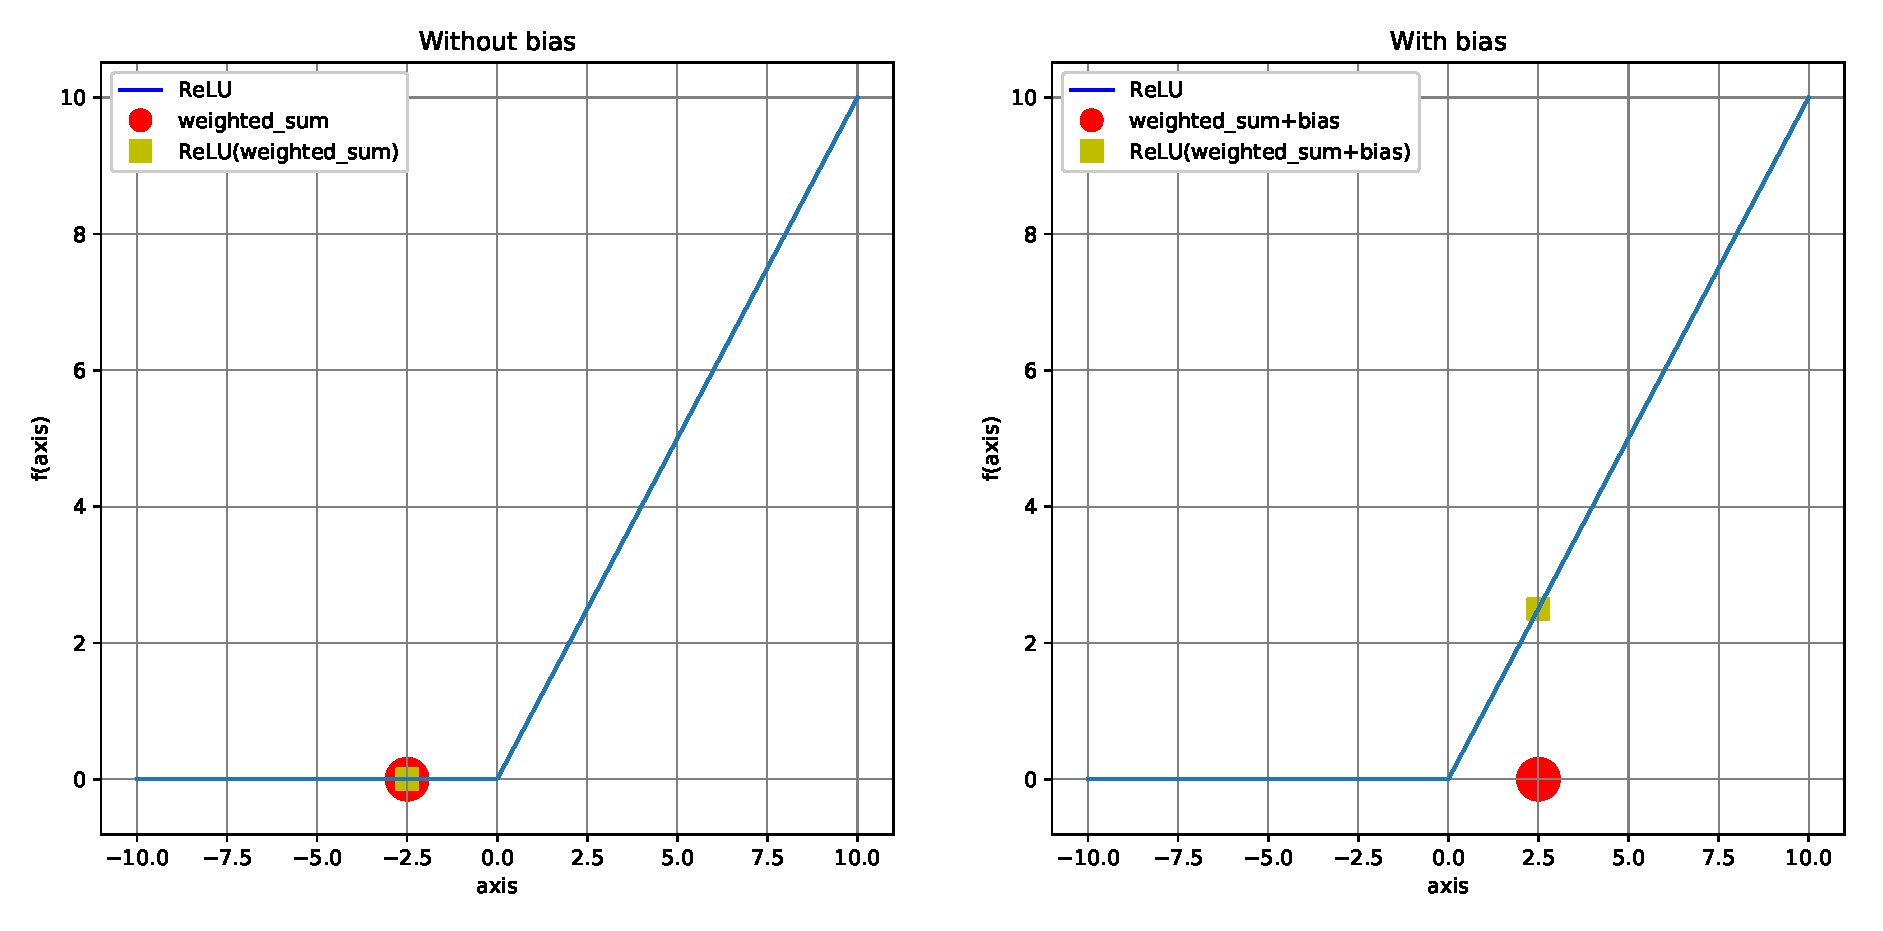
\includegraphics[width=0.95\textwidth]{Images/Plot/ReLU_bias.eps} 
\end{figure}
\end{frame}

\section{Xception}
\subsection{Architecture}
\begin{frame}
\frametitle{Xception}
\framesubtitle{Architecture} 

\begin{textblock}{15}(7.67,-0.62)
	\begin{figure}[H]
		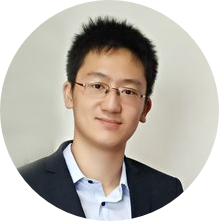
\includegraphics[width=0.1\textwidth]{Images/Team/WeihaoZHOU.png} 
	\end{figure}
\end{textblock}

\begin{textblock}{1}(8.1,1.2)
	\centerline{71 trainable layers ; 22,910,480 parameters}
\end{textblock}

\begin{center}
	
	{\fontsize{8.5}{8}\selectfont
		\begin{tabular}{ccccc}
			\textbf{Layer} & \textbf{Type} & \textbf{Activation function} & \textbf{Output Shape} & \textbf{Param} \\
			input\_1  & (\textcolor{gray}{InputLayer}) & N/A & (299, 299, 3) & \colorbox{yellow}{0} \\         
			block1\_conv1 & (\textcolor{orange}{Conv2D}) & N/A & (149, 149, 32) & 864 \\      
			block1\_conv1\_bn & (\textcolor{red}{Batch Normalization}) & N/A & (149, 149, 32) & 128 \\     
			block1\_conv1\_act & (\textcolor{cyan}{Activation}) & ReLU & (149, 149, 32) & \colorbox{yellow}{0} \\         
			block1\_conv2 & (\textcolor{orange}{Conv2D}) & N/A & (147, 147, 64) & 18,432 \\     
			block1\_conv2\_bn & (\textcolor{red}{Batch Normalization}) & N/A & (147, 147, 64) & 256 \\    
			block1\_conv2\_act & (\textcolor{cyan}{Activation}) & ReLU & (147, 147, 64) & \colorbox{yellow}{0} \\         
			\colorbox{gray}{block2...} & (...) & ... & (147, 147, 128) & ... \\   
			conv2d\_45 & (\textcolor{orange}{Conv2D}) & N/A & (74,74,128) & 8192 \\
			block2\_pool & (\textcolor{blue}{MaxPooling2D}) & N/A & (74,74,128) & \colorbox{yellow}{0} \\
			bn\_45 & (\textcolor{red}{Batch Normalization}) & N/A &(74,74,128) & 512 \\
			add & (\textcolor{violet}{Add}) & N/A & (74,74,128) & \colorbox{yellow}{0} \\
			\colorbox{gray}{block3...} & (...) & ... & (74, 74, 256) & ... \\    
			... & (...) & ... & (...) & ... \\    
			\colorbox{gray}{block14...} & (...) & ... & (10, 10, 1536) & 1,582,080 \\         
			        
			avg\_pool & (\textcolor{blue}{GlobalAveragePooling2D}) & N/A & (, 2048) & \colorbox{yellow}{0} \\          
			predictions & (\textcolor{green}{Dense}) & \textcolor{red}{Softmax} & (, 1000) & 2,049,000   
		\end{tabular}
	}
\end{center}
\end{frame}

\begin{frame}
\frametitle{Xception}
\framesubtitle{Transfer Learning} 

\begin{textblock}{15}(7.67,-0.62)
	\begin{figure}[H]
		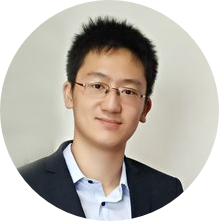
\includegraphics[width=0.1\textwidth]{Images/Team/WeihaoZHOU.png} 
	\end{figure}
\end{textblock}

\begin{center}
	{\fontsize{8.5}{8}\selectfont
		\begin{tabular}{@{\hspace{-0.2cm}}cccc}
			& \textbf{Layer Type} &\textbf{Activation function} & \textbf{Output Shape} \\
			& & \textcolor{white}{phantom} & \\
			\begin{tabular}{c}
				freeze weights\\ learned on ImageNet
			\end{tabular}	
			& $\left\{\begin{tabular}{c}
			(\textcolor{gray}{InputLayer}) \\         
			(\textcolor{orange}{Conv2D}) \\      
			(\textcolor{red}{Batch Normalization}) \\     
			(\textcolor{cyan}{Activation}) \\          
			(...)\\ 
			(...)\\      
			(\textcolor{blue}{GlobalAveragePooling2D}) \\         
			(\textcolor{green}{Dense}) \\ 
			\end{tabular}
			\right.\kern-\nulldelimiterspace$
			& \begin{tabular}{c}
				N/A \\
				N/A \\
				N/A \\
				ReLU \\
				...\\
				...\\
				N/A \\
				ReLU \\
			\end{tabular}
			& \begin{tabular}{c}
				(299, 299, 3) \\
				(149, 149, 32) \\
				(149, 149, 32) \\
				(149, 149, 32) \\
				(...)\\
				(...)\\
				(, 2048) \\
			\end{tabular} \\
			& \hspace{0.2cm} \sout{(\textcolor{green}{Dense})} & \sout{\textcolor{red}{Softmax}} & \sout{(, 1000)} \\
			\only<2>{& \hspace{0.2cm} \textcolor{magenta}{(Dropout)} & N/A & (, 2048) \\} 
			train this layer & \hspace{-1.2cm} $\left\{\begin{tabular}{c}
			\hspace{1.2cm} (\textcolor{green}{Dense})
			\end{tabular} \right.\kern-\nulldelimiterspace$ & \textcolor{red}{Softmax} & \hspace{0.1cm} (, nbClasses)
		\end{tabular}
	}
\end{center}
Trainable params: 6,147
\end{frame}

\section{VGG-16}
\definecolor{red}{rgb}{1,0,0}
\definecolor{green}{rgb}{0,0.39,0}
\renewcommand{\arraystretch}{1.1}

\subsection{Architecture}
\begin{frame}
\frametitle{VGG-16}
\framesubtitle{Architecture (2014)} 

\begin{textblock}{15}(7.67,-0.62)
	\begin{figure}[H]
		
\includegraphics[width=0.1\textwidth]{Images/Team/DamienTOOMEY.png} 
	\end{figure}
\end{textblock}

\begin{textblock}{1}(8.35,1)
	\centerline{16 trainable layers ; 138,357,544 parameters}
\end{textblock}

\begin{center}

{\fontsize{8.5}{0}\selectfont
\begin{tabular}{ccccc}
\textbf{Layer} & \textbf{Type} & \textbf{Activation function} & \textbf{Output Shape} & \textbf{Param} \\
input\_1  & (\textcolor{gray}{InputLayer}) & N/A & (224, 224, 3) & \colorbox{yellow}{0} \\         
block1\_conv1 & (\textcolor{orange}{Conv2D}) & ReLU & (224, 224, 64) & 1,792 \\      
block1\_conv2 & (\textcolor{orange}{Conv2D}) & ReLU & (224, 224, 64) & 36,928 \\     
block1\_pool & (\textcolor{blue}{MaxPooling2D}) & N/A & (112, 112, 64) & \colorbox{yellow}{0} \\         
block2\_conv1 & (\textcolor{orange}{Conv2D}) & ReLU & (112, 112, 128) & 73,856 \\     
block2\_conv2 & (\textcolor{orange}{Conv2D}) & ReLU & (112, 112, 128) & 147,584 \\    
block2\_pool & (\textcolor{blue}{MaxPooling2D}) & N/A & (56, 56, 128) & \colorbox{yellow}{0} \\         
block3\_conv1 & (\textcolor{orange}{Conv2D}) & ReLU & (56, 56, 256) & 295,168 \\    
block3\_conv2 & (\textcolor{orange}{Conv2D}) & ReLU & (56, 56, 256) & 590,080 \\    
block3\_conv3 & (\textcolor{orange}{Conv2D}) & ReLU & (56, 56, 256) & 590,080 \\    
block3\_pool & (\textcolor{blue}{MaxPooling2D}) & N/A & (28, 28, 256) & \colorbox{yellow}{0} \\         
block4\_conv1 & (\textcolor{orange}{Conv2D}) & ReLU & (28, 28, 512) & 118,0160 \\   
block4\_conv2 & (\textcolor{orange}{Conv2D}) & ReLU & (28, 28, 512) & 2,359,808 \\   
block4\_conv3 & (\textcolor{orange}{Conv2D}) & ReLU & (28, 28, 512) & 2,35,9808 \\   
block4\_pool & (\textcolor{blue}{MaxPooling2D}) & N/A & (14, 14, 512) & \colorbox{yellow}{0} \\         
block5\_conv1 & (\textcolor{orange}{Conv2D}) & ReLU & (14, 14, 512) & 2,359,808 \\   
block5\_conv2 & (\textcolor{orange}{Conv2D}) & ReLU & (14, 14, 512) & 2,359,808 \\   
block5\_conv3 & (\textcolor{orange}{Conv2D}) & ReLU & (14, 14, 512) & 2,359,808 \\   
block5\_pool & (\textcolor{blue}{MaxPooling2D}) & N/A & (7, 7, 512) & \colorbox{yellow}{0} \\         
flatten & (Flatten) & N/A & (, 25088) & \colorbox{yellow}{0} \\         
fc1 & (\textcolor{green}{Dense}) & ReLU & (, 4096) & \colorbox{magenta}{102,764,544} \\ 
fc2 & (\textcolor{green}{Dense}) & ReLU & (, 4096) & 16,781,312 \\  
predictions & (\textcolor{green}{Dense}) & \textcolor{red}{Softmax} & (, 1000) & 4,097,000   
\end{tabular}
}
\end{center}
\end{frame}

\begin{frame}
\frametitle{VGG-16}
\framesubtitle{Transfer Learning} 

\begin{textblock}{15}(7.67,-0.62)
	\begin{figure}[H]
		
\includegraphics[width=0.1\textwidth]{Images/Team/DamienTOOMEY.png} 
	\end{figure}
\end{textblock}

\vspace{-0.7cm}
\begin{center}
{\fontsize{8.5}{8}\selectfont
\begin{tabular}{@{\hspace{-0.2cm}}cccc}
& \textbf{Layer Type} &\textbf{Activation function} & \textbf{Output Shape} \\
& & \textcolor{white}{phantom} & \\
	\begin{tabular}{c}
	freeze weights\\ learned on ImageNet
	\end{tabular}	
	& $\left\{\begin{tabular}{c}
	(\textcolor{gray}{InputLayer}) \\         
	(\textcolor{orange}{Conv2D}) \\      
	(\textcolor{orange}{Conv2D}) \\     
	(\textcolor{blue}{MaxPooling2D}) \\         
	(\textcolor{orange}{Conv2D}) \\     
	(\textcolor{orange}{Conv2D}) \\    
	(\textcolor{blue}{MaxPooling2D}) \\         
	(\textcolor{orange}{Conv2D}) \\    
	(\textcolor{orange}{Conv2D}) \\    
	(\textcolor{orange}{Conv2D}) \\    
	(\textcolor{blue}{MaxPooling2D}) \\         
	(\textcolor{orange}{Conv2D}) \\   
	(\textcolor{orange}{Conv2D}) \\   
	(\textcolor{orange}{Conv2D}) \\   
	(\textcolor{blue}{MaxPooling2D}) \\         
	(\textcolor{orange}{Conv2D}) \\   
	(\textcolor{orange}{Conv2D}) \\   
	(\textcolor{orange}{Conv2D})  \\   
	(\textcolor{blue}{MaxPooling2D})\\         
	(Flatten) \\         
	(\textcolor{green}{Dense}) \\ 
	(\textcolor{green}{Dense}) \\
	\end{tabular}
	\right.\kern-\nulldelimiterspace$
	& \begin{tabular}{c}
	N/A \\
	ReLU \\
	ReLU \\
	N/A \\
	ReLU \\
	ReLU \\
	N/A \\
	ReLU \\
	ReLU \\
	ReLU \\
	N/A \\
	ReLU \\
	ReLU \\
	ReLU \\
	N/A \\
	ReLU \\
	ReLU \\
	ReLU \\
	N/A \\
	N/A \\
	ReLU \\
	ReLU \\	
	\end{tabular}
	& \begin{tabular}{c}
	(224, 224, 3) \\
	(224, 224, 64) \\
	(224, 224, 64) \\
	(112, 112, 64) \\
	(112, 112, 128) \\
	(112, 112, 128) \\
	(56, 56, 128) \\
	(56, 56, 256) \\
	(56, 56, 256) \\
	(56, 56, 256) \\
	(28, 28, 256) \\ 
	(28, 28, 512) \\
	(28, 28, 512) \\
	(28, 28, 512) \\
	(14, 14, 512) \\
	(14, 14, 512) \\
	(14, 14, 512) \\
	(14, 14, 512) \\
	(7, 7, 512) \\
	(, 25088) \\
	(, 4096) \\
	(, 4096) \\
	\end{tabular} \\
	& \hspace{0.2cm} \sout{(\textcolor{green}{Dense})} & \sout{\textcolor{red}{Softmax}} & \sout{(, 1000)} \\
	\only<2>{& \hspace{0.2cm} \textcolor{magenta}{(Dropout)} & N/A & (, 4096) \\} 
	train this layer & \hspace{-0.5cm} $\left\{\begin{tabular}{c}
	\hspace{0.5cm} (\textcolor{green}{Dense})
	\end{tabular} \right.\kern-\nulldelimiterspace$ & \textcolor{red}{Softmax} & \hspace{0.1cm} (, nbClasses)
\end{tabular}
}
\end{center}

\end{frame}


\section{ResNet-50}
\definecolor{red}{rgb}{1,0,0}
\definecolor{green}{rgb}{0,0.39,0}
\renewcommand{\arraystretch}{1.1}

\subsection{Architecture}
\begin{frame}
\frametitle{RESNET-50}
\framesubtitle{Architecture (2015)} 

\begin{textblock}{15}(7.67,-0.62)
	\begin{figure}[H]
		
\includegraphics[width=0.1\textwidth]{Images/Team/MehdiABOUZAID.png} 
	\end{figure}
\end{textblock}

\begin{textblock}{1}(8.7,1)
	\centerline{50 trainable layers ; 25,636,712 parameters}
\end{textblock}

\begin{center}
	
	{\fontsize{7.5}{0}\selectfont
		\begin{tabular}{ccccc}
			
			\textbf{Layer} & \textbf{Type} & \textbf{Activation function} & \textbf{Output Shape} & \textbf{Param} \\
			input\_1  & (\textcolor{gray}{InputLayer}) & N/A & (224, 224, 3) & \colorbox{yellow}{0} \\             
			res..\_branch.. & (\textcolor{orange}{Conv2D}) & N/A & (112, 112, 64) & 9,472 \\    
			bn..\_branch.. & (\textcolor{red}{Batch Normalization}) & N/A & (112, 112, 64) & 256 \\     
			activation\_.. & (\textcolor{cyan}{Activation}) & ReLU & (112, 112, 64) & \colorbox{yellow}{0} \\
			max\_pooling2d\_1 & (\textcolor{blue}{MaxPooling2D}) & N/A & (56, 56, 64) & \colorbox{yellow}{0} \\     
			
			res..\_branch.. & (\textcolor{orange}{Conv2D}) & N/A & (56, 56, 64) &  4,160 \\ 
			bn..\_branch..  & (\textcolor{red}{Batch Normalization}) & N/A & (56, 56, 64) & 256 \\ 
			activation\_.. & (\textcolor{cyan}{Activation}) & ReLU & (56, 56, 64) & \colorbox{yellow}{0} \\
			res..\_branch.. & (\textcolor{orange}{Conv2D}) & N/A & (56, 56, 64) & 36,928 \\ 
			bn..\_branch..  & (\textcolor{red}{Batch Normalization}) & N/A & (56, 56, 64) & 256 \\          
			activation\_.. & (\textcolor{cyan}{Activation}) & ReLU & (56, 56, 64) & \colorbox{yellow}{0} \\
			res..\_branch.. & (\textcolor{orange}{Conv2D}) & N/A & (56, 56, 256) & 16,640 \\ 
			bn..\_branch..  & (\textcolor{red}{Batch Normalization}) & N/A & (56, 56, 256) & 256 \\ 
			activation\_.. & (\textcolor{cyan}{Activation}) & ReLU & (56, 56, 64) & \colorbox{yellow}{0} \\
			& ... & & &\\
			res..\_branch.. & (\textcolor{orange}{Conv2D}) & ReLU & (28, 28, 128) & 32,896 \\ 
			& ... & & &\\   
			res..\_branch.. & (\textcolor{orange}{Conv2D}) & ReLU & (28, 28, 128) & 147,584 \\         
			res..\_branch.. & (\textcolor{orange}{Conv2D}) & ReLU & (28, 28, 512) & 66,048 \\   
			
			res..\_branch.. & (\textcolor{orange}{Conv2D}) & ReLU & (14, 14, 256) & 131,328 \\   
			res..\_branch.. & (\textcolor{orange}{Conv2D}) & ReLU & (14, 14, 256) &  590,080  \\         
			res..\_branch.. & (\textcolor{orange}{Conv2D}) & ReLU & (14, 14, 1024) & 263,168 \\  
			
			res..\_branch.. & (\textcolor{orange}{Conv2D}) & ReLU & (7, 7, 512) & 524,800 \\   
			res..\_branch.. & (\textcolor{orange}{Conv2D}) & ReLU & (7, 7, 512) & 2,359,808 \\   
			res..\_branch.. & (\textcolor{orange}{Conv2D}) & ReLU & (7, 7, 2048) & 1,050,624 \\
			
			
			avg\_pool & (\textcolor{blue}{GlobalAveragePooling2D}) & N/A & (,2048) & \colorbox{yellow}{0} \\         
			fc1000 & (\textcolor{green}{Dense}) & SoftMax & (, 1000) & \colorbox{magenta}{2,049,000} \\ 
			
		\end{tabular}
	}
\end{center}
\end{frame}





\begin{frame}
\frametitle{RESNET-50}
\framesubtitle{Transfer Learning} 

\begin{textblock}{15}(7.67,-0.62)
\begin{figure}[H]
	
\includegraphics[width=0.1\textwidth]{Images/Team/MehdiABOUZAID.png} 
\end{figure}
\end{textblock}

\begin{center}
{\fontsize{8.5}{6.5}\selectfont
	\begin{tabular}{@{\hspace{-0.2cm}}cccc}
		& \textbf{Layer Type} &\textbf{Activation function} & \textbf{Output Shape} \\
		& & \textcolor{white}{phantom} & \\
		\begin{tabular}{c}
			freeze weights\\ learned on ImageNet
		\end{tabular}	
		& $\left\{\begin{tabular}{c}
		(\textcolor{gray}{InputLayer}) \\         
		(\textcolor{orange}{Conv2D}) \\      
		
		(\textcolor{blue}{MaxPooling2D}) \\         
		(\textcolor{orange}{Conv2D}) \\     
		(\textcolor{orange}{Conv2D}) \\             
		(\textcolor{orange}{Conv2D}) \\    
		(\textcolor{orange}{Conv2D}) \\    
		(\textcolor{orange}{Conv2D}) \\            
		(\textcolor{orange}{Conv2D}) \\   
		(\textcolor{orange}{Conv2D}) \\   
		(\textcolor{orange}{Conv2D}) \\        
		(\textcolor{orange}{Conv2D}) \\   
		(\textcolor{orange}{Conv2D}) \\  
		(\textcolor{orange}{Conv2D}) \\   
		(\textcolor{orange}{Conv2D})  \\   
		(\textcolor{blue}{GlobalAveragePooling2D})\\  
		\end{tabular}
		\right.\kern-\nulldelimiterspace$
		& \begin{tabular}{c}
			N/A \\
			ReLU \\
			ReLU \\
			ReLU \\
			ReLU \\
			ReLU \\
			ReLU \\
			ReLU \\
			ReLU \\
			ReLU \\
			ReLU \\
			ReLU \\
			ReLU \\
			ReLU \\
			ReLU \\
			ReLU \\
			ReLU \\	
		\end{tabular}
		& \begin{tabular}{c}
			(224,224,3) \\
			(112, 112, 64) \\
			(56, 56, 64) \\
			(56, 56, 64) \\
			(56, 56, 64) \\
			(56, 56, 256) \\
			(28, 28 , 128) \\
			(28, 28, 128) \\
			(28, 28, 512) \\
			(14, 14, 256) \\
			(14, 14, 256) \\
			(14, 14, 1024) \\ 
			(7, 7, 512) \\
			(7, 7, 512) \\
			(7, 7, 2048) \\
			(,2048)
		\end{tabular} \\
		& \hspace{0.2cm} \sout{(\textcolor{green}{Dense})} & \sout{\textcolor{red}{Softmax}} & \sout{(, 1000)} \\
		\only<2>{& \hspace{0.2cm} \textcolor{magenta}{(Dropout)} & N/A & (, 2048) \\} 
		train this layer & \hspace{-0.5cm} $\left\{\begin{tabular}{c}
		\hspace{0.5cm} (\textcolor{green}{Dense})
		\end{tabular} \right.\kern-\nulldelimiterspace$ & \textcolor{red}{Softmax} & \hspace{0.1cm} (, nbClasses)
	\end{tabular}
}
\end{center}
Trainable params: 6,147
\end{frame}


\section{Conclusion}
\subsection{Our results}
\begin{frame}
\frametitle{Conclusion}
\framesubtitle{Our results}

\begin{textblock}{15}(7.67,-0.62)
	\begin{figure}[H]
		
\includegraphics[width=0.1\textwidth]{Images/Team/DamienTOOMEY.png} 
	\end{figure}
\end{textblock}

\begin{figure}[H]
	
\includegraphics[width=1\textwidth]{Images/quote_yann_lecun.png} 
\end{figure}

\end{frame}


\subsection{Our results}
\begin{frame}
\frametitle{Conclusion}
\framesubtitle{Our results}

\begin{textblock}{15}(7.67,-0.62)
	\begin{figure}[H]
		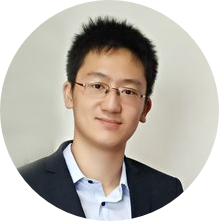
\includegraphics[width=0.1\textwidth]{Images/Team/WeihaoZHOU.png} 
	\end{figure}
\end{textblock}

\setlength{\tabcolsep}{1pt}

\begin{adjustwidth}{-1.5em}{-1.5em}
\begin{center}

{\fontsize{7}{11}\selectfont

\textbf{\textcolor{blue}{Training set} (3867 images)}
\vspace{0.5cm}

\begin{tabular}{|c||c|c|c?c|c|c?c|c|c?c|c|c|}
\cline{2-13}
\multicolumn{1}{c|}{} & \multicolumn{12}{c|}{\textbf{\textcolor{blue}{Validation set} (967 images)} : Top 1 Accuracy} \\
\cline{2-13}
\multicolumn{1}{c|}{} & \multicolumn{6}{c?}{With 0.5 dropout} & \multicolumn{6}{c|}{Without dropout} \\
\hline
Epochs & \multicolumn{3}{c?}{2} & \multicolumn{3}{c?}{10} & \multicolumn{3}{c?}{2} & \multicolumn{3}{c|}{10} \\
\hline
Batch size & 8 & 16 & 32 & 8 & 16 & 32 & 8 & 16 & 32 & 8 & 16 & 32 \\
\noalign{\global\arrayrulewidth=1pt} \hline \noalign{\global\arrayrulewidth=0.4pt}
Xception & 0.3588 & 0.3661 & 0.3609 & 0.3909 & 0.3433 & 0.3454 & 0.4116 & 0.4012 & 0.4012 & \colorbox{yellow}{0.4199} & 0.3899 & 0.3733 \\
\hline
VGG-16 & 0.9741 & 0.9835 & 0.9824 & 0.9824 & 0.9855 & 0.9824 & 0.9762 & 0.9845 & \colorbox{yellow}{0.9866} & 0.9814 & 0.9814 & 0.9814 \\
\hline
ResNet-50 & 0.9659 & 0.9700 & 0.9721 & 0.9731 & \colorbox{yellow}{0.9741} & 0.9731 & 0.9690 & 0.9690 & 0.9659 & 0.9710 & 0.9710 & 0.9710 \\
\hline
\multicolumn{13}{c}{\textcolor{white}{phantom}} \\
\cline{2-13}
\multicolumn{1}{c|}{} & \multicolumn{12}{c|}{\textbf{\textcolor{blue}{Test set} (1209 images)} : Top 1 Accuracy} \\
\cline{2-13}
\multicolumn{1}{c|}{} & \multicolumn{6}{c?}{With 0.5 dropout} & \multicolumn{6}{c|}{Without dropout} \\
\hline
Epochs & \multicolumn{3}{c?}{2} & \multicolumn{3}{c?}{10} & \multicolumn{3}{c?}{2} & \multicolumn{3}{c|}{10} \\
\hline
Batch size & 8 & 16 & 32 & 8 & 16 & 32 & 8 & 16 & 32 & 8 & 16 & 32 \\
\noalign{\global\arrayrulewidth=1pt} \hline \noalign{\global\arrayrulewidth=0.4pt}
Xception & 0.3524 & 0.3677 & 0.3490 & \colorbox{yellow}{0.4030} & 0.3711 & 0.3708 & 0.3984 & 0.3764 & 0.3423 & 0.3667 & 0.3422 & 0.3598 \\
\hline
VGG-16 & 0.9586 & 0.9702 & 0.9727 & 0.9644 & 0.9702 & \colorbox{yellow}{0.9744} & 0.9628 & 0.9686 & 0.9653 & 0.9669 & 0.9694 & 0.9686 \\
\hline
ResNet-50 & 0.9661 & 0.9661 & 0.9711 & 0.9702 & 0.9735 & 0.9711 & 0.9686 & \colorbox{yellow}{0.9694} & \colorbox{yellow}{0.9694} & 0.9537 & 0.9644 & 0.9639 \\
\hline
\end{tabular}
}
\end{center}

\end{adjustwidth}

\end{frame}


\section{References}
\begin{frame}
\frametitle{References}
	
\begin{myitemize}
\item[•] Stanford University School of Engineering
	\begin{myitemize}
		\item[-] Lecture 5 $\vert$ Convolutional Neural Networks
		\item[] \url{https://www.youtube.com/watch?v=bNb2fEVKeEo}
		\item[-] Lecture 7 $\vert$ Training Neural Networks II
		\item[] \url{https://www.youtube.com/watch?v=_JB0AO7QxSA} (1h12min : transfer learning)
		\item[-] Lecture 9 $\vert$ CNN Architectures
		\item[] \url{https://www.youtube.com/watch?v=DAOcjicFr1Y}
		\item[-] CS231n Convolutional Neural Networks for Visual Recognition
		\item[] \url{http://cs231n.github.io/convolutional-networks/}
	\end{myitemize}
\item[•] MIT OpenCourseWare
	\begin{myitemize}
		\item[-] 12a: Neural Nets
		\item[] \url{https://www.youtube.com/watch?v=uXt8qF2Zzfo} {bias: 23min}
		\item[-] 12b: Deep Neural Nets
		\item[] \url{https://www.youtube.com/watch?v=VrMHA3yX_QI} (kernels = neurone: 12min; softmax explanation: 34min)
	\end{myitemize}
\end{myitemize}
\end{frame}

\begin{frame}
\frametitle{References}
	
\begin{myitemize}
\item[•] AlexNet Original Article:
\item[] \url{https://papers.nips.cc/paper/4824-imagenet-classification-with-deep-convolutional-neural-networks.pdf}
\item[•] VGG-16 Original article : VERY DEEP CONVOLUTIONAL NETWORKS FOR LARGE-SCALE IMAGE RECOGNITION
\item[] \url{https://arxiv.org/pdf/1409.1556.pdf}
\item[•] VGG-16: "The only preprocessing we do is subtracting the mean RGB value, computed on the training set, from each pixel."
\item[] \url{https://machinelearningmastery.com/use-pre-trained-vgg-model-classify-objects-photographs/})
\item[•] Batch Normalization : learnable parameters
\item[] \url{https://medium.com/coinmonks/paper-review-of-alexnet-caffenet-winner-in-ilsvrc-2012-image-classification-b93598314160}
\item[•] Keras pretrained Models
\item[] \url{https://keras.io/applications/}
\item[•] Pretrained Deep Neural Networks Matlab
\item[•] \url{https://www.mathworks.com/help/deeplearning/ug/pretrained-convolutional-neural-networks.html}


\end{myitemize}
\end{frame}

\end{document}